\section{Лабораторная работа 4 }
\textbf{Тема:}Определение энергии активации и порядка реакции разложения пероксида водорода.

\textbf{Цель работы:}газометрическим методом определить порядок и энергию активации реакции разложении пероксида водорода ($H_{2}O_{2}$).

\textbf{Оборудование и реактивы:} установка для изучения разложения $H_{2}O_{2}$, термостат, термометр, пробирки на 20 - 25 мл., раствор $CuSO_{4}$ (1 Н), раствор пероксида водорода (4\%), $MnO_{2}$, вода.

\textbf{Теория}
\textit{\textbf{1. Определение порядка реакции.}}

Пероксид водорода в водных растворах самопроизвольно разлагается по уравнению:
$$H_{2}O_{2}\rightarrow H_{2}O+0.5O_{2}\uparrow$$
В присутствии некоторых веществ разложение пероксида водорода значительно ускоряется. В данной работе катализаторами могут быть сульфат меди или оксид марганца(IV).

Поскольку и $CuSO_{4}$, и $H_{2}O_{2}$ находятся в водном растворе (одна фаза), эта реакция является гомогенной каталитической реакцией. Оксид марганца (IV) используется в виде порошка (две фазы), тогда реакция является гетерогенной каталитической.

$$r=kC^{x},$$
где $C$ -- концентрация пероксида водорода, моль/л;

$k$ -- кинетическая константа реакции;

$x$ -- порядок реакции.

Для определения величин порядка реакции и кинетической константы построим график в координатах $ln(r)$ --- $ln(C)$. 
$$ln(r)=ln(k)+x\cdot ln(C)$$
Тогда порядок реакции определится как тангенс угла наклона прямой, а $ln(k)$ --- по отрезку, отсекаемому прямой на вертикальной оси.
Концентрация пероксида водорода может быть расчитана по формуле:
$$C=\frac{n_{01}-X}{V}=C_{0}-\frac{X}{V_{1}},$$
где $n_{01}$ -- начальное количество пероксида водорода,моль;

$X$ -- количество прореагировавшего пероксида водорода, моль;

$C_{0}$ -- начальная концентрация пероксида водорода, моль/л.

$V_{1}$ -- объем реакционной смеси, л.

Величину $X$ определим из реакции через объем выделившегося кислорода. Последний свяжем с количеством вещества через уравнение Менделеева-Клапейрона.
$$PV=n_{3}RT,$$
$$X=2n_{3}=\frac{2PV}{RT}=\frac{2\cdot 101325\cdot V}{8,31\cdot 298}=81,83V$$
$P$ -- давление, Па;

$V$ -- объем выделившегося кислорода, м~$^{3}$;

$n_{3}$ -- количество выделившегося кислорода, моль;

$R$ -- газовая постоянная;

$T$ -- температура, К.

Тогда: 
$$C=C_{0}-0,082\cdot\frac{V}{V_{1}}$$
Среднюю скорость реакции расчитаем по формуле:
$$r=\frac{\Delta C}{\Delta\tau}=\frac{0,082V}{V_{1}\cdot\Delta\tau}$$
где $\Delta\tau$ -- интервал времени, мин.

Величину начальной молярной концентрации пероксида водорода определить по таблице 1. Объемы в формулах (1), (2) брать в миллилитрах.

\begin{table}[h]
\caption{Плотности растворов пероксида водорода ($M=34,01$г/Моль) при 18~$^{o}$~C}
\label{tabular:data22_1}
\begin{center}
\begin{tabular}{|p{5cm}|p{5cm}|}
\hline
Массовая доля, \% & Плотность, г/мл \\
\hline
1 & 1,0022\\
\hline
2 & 1,0058\\
\hline
4 & 1,0131\\
\hline
6 & 1,0204\\
\hline
8 & 1,0277\\
\hline
10 & 1,0351\\
\hline
\end{tabular}
\end{center}
\end{table}

\textit{\textbf{2. Определение порядка реакции по уравнениям кинетических констант}}

Величину порядка реакции и кинетической константы можно определить по известным уравнениям для кинетических констант реакции порядка 0, 1, 2, 3, ...

Для этого по уравнениям из таблицы \ref{tabular:data22_2} для кинетических констант реакций различных порядков рассчитывают величины констант для каждого момента времени по экспериментальным данным. Если реакция имеет целочисленный порядок, то соответствующая расчетная величина константы будет сохранять постоянство на всем интервале измерения.
\begin{table}[h!]
\caption{Кинетические характеристики реакций 1-го, 2-го и 3-го порядков}
\label{tabular:data22_2}
\begin{center}
\begin{tabular}{|>{\centering\arraybackslash}p{0.1\linewidth}|>{\centering\arraybackslash}p{0.15\linewidth}|>{\centering\arraybackslash}p{0.25\linewidth}|>{\centering\arraybackslash}p{0.2\linewidth}|>{\centering\arraybackslash}p{0.15\linewidth}|}
\hline 
Порядок реакции (общий) &
Дифферен-\- циальное уравнение $r=r(C,T)$, размерность кинетической константы $[k]$ &
Интегральное уравнение, $C=C(\tau,T)$ выражение для кинетической константы $k$&
Степень превращения $\alpha=\frac{C_{0}-C}{C_{0}}$&
Время полупревращения, $\tau_{0,5}$ ($\alpha=0,5$, $C=0,5C_{0}$)
\\ 
\hline 
0 & $$-\frac{dC}{d\tau}=k$$ 
$$[k]=\frac{\textsc{моль}}{\textsc{м}^{3}\textsc{с}}$$& 
$$C=C_{0}-k\tau$$ 
$$k=\frac{C_{0}-C}{\tau}$$ &
$$\alpha=\frac{k\tau}{C_{0}}$$ & 
$$\tau_{0,5}=\frac{C_{0}}{2k}$$\\ 
\hline 
1 &  $$-\frac{dC}{d\tau}=kC$$ 
$$[k]=\textsc{с}^{-1}$$&
$$ln(C)=ln(C_{0})-k\tau$$
$$k=\frac{1}{\tau}\cdot ln\left(\frac{C_{0}}{C}\right)$$&
$$\alpha=1-e^{-k\tau}$$ &
$$\tau_{0,5}=\frac{ln(2)}{2k}$$\\ 
\hline 
2 &  $$-\frac{dC}{d\tau}=kC^{2}$$ 
$$[k]=\frac{\textsc{м}^{3}}{\textsc{моль}\textsc{с}}$$&
$$\frac{1}{C}=\frac{1}{C_{0}}+k\tau$$
$$k=\frac{1}{\tau}\cdot\left(\frac{1}{C}-\frac{1}{C_{0}}\right)$$&
$$\alpha=\frac{k\tau C_{0}}{k\tau C_{0}+1}$$&
$$\tau_{0,5}=\frac{1}{kC_{0}}$$\\ 
\hline 
3 & $$-\frac{dC}{d\tau}=kC^{3}$$ 
$$[k]=\frac{(\textsc{м}^{3})^{2}}{\textsc{моль}^{2}\textsc{с}}$$&
$$\frac{1}{C^{2}}=\frac{1}{C_{0}^{2}}+2k\tau$$
$$k=\frac{1}{2\tau}\cdot\left(\frac{1}{C^{2}}-\frac{1}{C_{0}^{2}}\right)$$&
$$k=\frac{\alpha(2-\alpha)}{2\tau C_{0}^{2}(1-\alpha)^{2}}$$&
$$\tau_{0,5}=\frac{3}{2kC_{0}}$$\\ 
\hline 
\end{tabular} 
\end{center}
\end{table}

\textit{\textbf{3. Определение энергии активации.}}

Зависимость константы скорости от температуры выражается уравнением Аррениуса:
$$ln(k)=ln(k_{0})-\frac{E}{R}\cdot\frac{1}{T},$$
где: $E$ -- энергия активации;

В координатах $ln(k)$ --- $\frac{1}{T}$ экспериментальные данные должны лежать на прямой. Её тангенс угла наклона $tg(\phi)$ находят из графика, а затем, вычисляют Е:
$$E=R\cdot tg(\phi)$$
Возможно также применение аналитического метода. Решаем систему уравнений Аррениуса относительно $E$ и $k_{0}$.
$$
\begin{cases}
ln(k_{1})= ln(k_{0})-\frac{E}{R}\cdot\frac{1}{T_{1}}\\
ln(k_{2})= ln(k_{0})-\frac{E}{R}\cdot\frac{1}{T_{2}}
\end{cases}
$$

Решение:
$$E=\frac{RT_{1}T_{2}}{T_{1}-T_{2}}ln\left(\frac{k_{1}}{k_{2}}\right)$$
$$k_{0}=\frac{T_{1}ln(k_{1})-T_{2}ln(k_{2})}{T_{1}-T_{2}}$$

\textbf{Порядок выполнения}
Наблюдение за ходом реакции и определение её скорости ведется путём измерения объёма выделившегося кислорода (газометрический метод). Измерения проводят через определенные промежутки времени от начала реакции. Прибор для работы (Рис. \ref{ris:image22_1}.) состоит из реакционной пробирки 1, бюретки 2 и уравнительного сосуда 3, соединённого резиновым шлангом с нижней частью измерительной бюретки.
Пробирка с реакционной смесью помещается в водяной термостат 4.

\begin{figure}[h]
\center{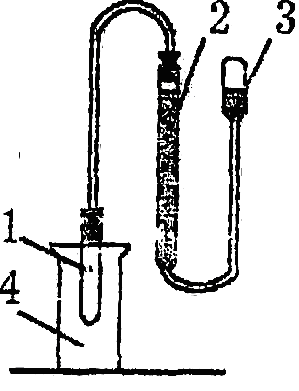
\includegraphics[width=0.25\linewidth]{volume.png}}
\caption{Схема экспериментальной установки}
\label{ris:image22_1}
\end{figure}
\underline{При использовании в качестве катализатора $CuSO_{4}$:}

В реакционную пробирку 1 наливают 10 мл раствора $CuSO_{4}$ (1 Н) и 10 мл дистиллированной воды; пробирку помещают в термостат. Передвигая уравнительный сосуд вверх и вниз, устанавливают уровень жидкости в бюретке на нуле. После 10-ти минутного термостатирования в смесь вливают 5 мл 4\% раствора $H_{2}O_{2}$, тщательно перемешивают, записывают время опыта и температуру. Общий объем жидкости 25 мл.

\underline{При использовании в качестве катализатора $MnO_{2}$:}

В реакционную пробирку 1 засыпают примерно 1 г $MnO_{2}$, заливают 10 мл дистиллированной воды; пробирку помещают в термостат. Передвигая уравнительный сосуд вверх и вниз, устанавливают уровень жидкости в бюретке на нуле. После 10-ти минутного термостатирования в смесь вливают 5 мл 4\% раствора $H_{2}O_{2}$, тщательно перемешивают, записывают время опыта и температуру. 

Выделяющийся кислород будет вытеснен из бюретки. Через определенные промежутки времени отсчитывают объем выделившегося кислорода. Реакция считается законченной, если уровень жидкости в бюретке перестанет опускаться. Результаты опыта записывают в таблицу \ref{tabular:data22_3}.

Первый опыт проводят при комнатной температуре. Затем повторяют опыт ещё 1 – 2 раза при других температурах. Таблица \ref{tabular:data22_3} заполняется отдельно для результатов при каждой температуре для каждого катализатора.

Рекомендуемые интервалы между отсчётами: при температуре термостата 20-25~$^{o}$~С --- интервал 5 минут; при температуре 30-40~$^{o}$~С --- 3 минуты. 

\begin{table}[h]
\caption{Экспериментальные данные}
\label{tabular:data22_3}
\begin{center}
\begin{tabular}{|p{0.15\linewidth}|p{0.4\linewidth}|p{0.4\linewidth}|}
\hline
\No\ измерения & Время от начала опыта, $\tau$, мин & Объём кислорода $V$, мл \\
\hline
& & \\
\hline
\end{tabular}
\end{center}
\end{table}

\textbf{Обработка экспериментальных данных}

\textit{\textbf{1. Определение порядка реакции.}}

Расчеты в таблицах \ref{tabular:data22_4}, \ref{tabular:data22_5} выполняются для всех серий измерений, для которых получены данные в таблице \ref{tabular:data22_3} (для всех катализаторов при различных температурах), при которых проводился эксперимент. Для каждой температуры следует заполнить указанные таблицы.

Заполнить таблицу \ref{tabular:data22_4}. Расчет выполняется по формулам (1), (2).
\begin{table}[h]
\caption{Результаты расчетов для определения порядка реакции дифференциальным методом}
\label{tabular:data22_4}
\begin{center}
\begin{tabular}{|p{0.15\linewidth}|p{0.15\linewidth}|p{0.15\linewidth}|p{0.22\linewidth}|p{0.22\linewidth}|}
\hline
\No\ измерения& $\tau$, мин & $C_{H_{2}O_{2}}$, моль/л & $ln(r)$ & $ln(C)$ \\
\hline 
 & & & & \\
\hline
\end{tabular}
\end{center}
\end{table}

Заполнить таблицу \ref{tabular:data22_5}. Расчет выполняется по формулам для кинетических констант 0-го, 1-го, 2-го, 3-го порядков из таблицы \ref{tabular:data22_2}.
\begin{table}[h]
\caption{Результаты расчета для определения порядка реакции интегральным методом}
\label{tabular:data22_5}
\begin{center}
\begin{tabular}{|p{0.15\linewidth}|p{0.15\linewidth}|p{0.15\linewidth}|p{0.1\linewidth}|p{0.1\linewidth}|p{0.1\linewidth}|p{0.1\linewidth}|}
\hline
\No\ измерения& $\tau$, мин & $C_{H_{2}O_{2}}$, моль/л & $k_{0}$ & $k_{1}$ & $k_{2}$ & $k_{3}$ \\
\hline 
 & & & & & & \\
\hline
\end{tabular}
\end{center}
\end{table}

\textit{\textbf{2. Определение энергии активации.}}

В случае использования графического метода заполняют таблицу \ref{tabular:data22_6} и строят график в координатах $ln(k)$---$\frac{1}{T}$.

Для выполнения расчета по уравнению Аррениуса можно воспользоваться формулами (3).

\begin{table}[h]
\caption{Результаты расчетов для определения параметров уравнения Аррениуса}
\label{tabular:data22_6}
\begin{center}
\begin{tabular}{|p{0.22\linewidth}|p{0.22\linewidth}|p{0.22\linewidth}|p{0.22\linewidth}|}
\hline
 $$T,$$ K& $$k$$ & $$ln(k)$$ & $$\frac{1}{T}$$ \\
\hline 
 & & & \\
\hline
\end{tabular}
\end{center}
\end{table}

\textbf{Контрольные вопросы}
\begin{enumerate}
\item Что называют скоростью химической реакции?
\item Что такое средняя и истинная скорость?
\item Какие факторы влияют на скорость химических реакций?
\item Сформулируйте закон действующий масс.
\item Что такое константа скорости химической реакции? 
\item Как зависит скорость химической реакции от температуры?
\item Что такое энергия активации? Какова зависимость между скоростью реакции и энергией активации?
\item Что такое молекулярность химической реакции?
\item Что такое порядок химической реакции?
\item В каких случаях молекулярность и порядок химической реакции не совпадают?
\item Какой вид имеет кинетическое уравнение химической реакции 1-го и 2-го и любого другого порядка?
\item На основании каких данных рассчитываются энергии активации?
\item Что называют катализом и катализатором? Какое влияние оказывает катализатор на энергию активации реакции?
\item Что такое гомогенный катализ? Механизм гомогенного катализа?
\item Гетерогенный катализ? Стадии гетерогенного катализа?
\item Методы ускорения гетерогенного катализа?
\end{enumerate}

